\section{Báo cáo chi tiết nội dung nghiên cứu và thực hiện}

\subsection{Dữ liệu nghiên cứu}
Dữ liệu đóng vai trò quyết định trong các bài toán điều khiển bằng dữ liệu (data-driven), đặc biệt là với các mô hình học sâu. Để xây dựng hệ thống giám sát biến động rừng tỉnh Cà Mau, nghiên cứu này đã thiết lập một quy trình thu thập và xử lý dữ liệu nghiêm ngặt từ các nguồn vệ tinh miễn phí nhưng chất lượng cao của Chương trình Copernicus.

\begin{figure}[H]
    \centering
    \includegraphics[width=0.95\textwidth]{img/chapter3/LULC-Ca-Mau.png}
    \caption{Bản đồ lớp phủ bề mặt khu vực tỉnh Cà Mau}
    \label{fig:camau_lulc}
\end{figure}

\subsubsection{Thu thập và tiền xử lý ảnh vệ tinh}
Nguồn dữ liệu chính được sử dụng bao gồm ảnh quang học từ vệ tinh Sentinel-2 và ảnh radar khẩu độ tổng hợp (SAR) từ vệ tinh Sentinel-1. Đối với Sentinel-2, nghiên cứu lựa chọn sản phẩm cấp độ L2A (Surface Reflectance) đã được hiệu chỉnh khí quyển để loại bỏ ảnh hưởng của sương mù và khí dung, đảm bảo giá trị phản xạ bề mặt chính xác. Các ảnh được thu thập trong giai đoạn mùa khô, cụ thể là tháng 01/2024 (kỳ trước) và tháng 02/2025 (kỳ sau), nhằm giảm thiểu tối đa sự che phủ của mây và đảm bảo tính tương đồng về điều kiện chiếu sáng giữa hai thời điểm. Toàn bộ quy trình truy xuất được thực hiện trên nền tảng điện toán đám mây Google Earth Engine (GEE), cho phép lọc và xử lý khối lượng lớn dữ liệu một cách hiệu quả. Các ảnh Sentinel-2 sau khi lọc mây với ngưỡng xác suất 50\% đã được dùng để tính toán các chỉ số thực vật quan trọng.

Song song đó, dữ liệu Sentinel-1 được thu thập ở chế độ Interferometric Wide (IW) với hai kênh phân cực VV và VH. Dữ liệu này được tiền xử lý các bước tiêu chuẩn gồm hiệu chỉnh quỹ đạo, khử nhiễu nhiệt, hiệu chỉnh bức xạ và hiệu chỉnh địa hình để tạo ra ảnh tán xạ ngược (backscatter) có đơn vị dB. Ưu điểm vượt trội của dữ liệu radar là khả năng xuyên thấu qua mây, cung cấp thông tin liên tục về cấu trúc bề mặt ngay cả khi dữ liệu quang học bị gián đoạn.

\subsubsection{Trích xuất đặc trưng}
Thay vì đưa trực tiếp ảnh thô vào mô hình, nghiên cứu đã tiến hành trích xuất một tập hợp các đặc trưng giàu thông tin nhằm nâng cao khả năng phân loại của mô hình. Tổng cộng 27 đặc trưng đã được xây dựng cho mỗi điểm ảnh. Từ dữ liệu Sentinel-2, bốn kênh phổ cơ bản gồm Blue (B2), Green (B3), Red (B4) và Near-Infrared (B8) cùng hai kênh hồng ngoại sóng ngắn (SWIR) được sử dụng. Bên cạnh đó, ba chỉ số thực vật chuyên biệt được tính toán gồm NDVI (chỉ số thực vật chuẩn hóa) phản ánh mật độ xanh, NBR (tỷ số cháy chuẩn hóa) nhạy cảm với sự mất mát sinh khối, và NDMI (chỉ số độ ẩm) phản ánh hàm lượng nước trong lá. Từ dữ liệu Sentinel-1, hai kênh phân cực VV và VH cung cấp thông tin về độ nhám và cấu trúc thể tích của tán rừng. Đặc biệt, để nắm bắt thông tin về sự thay đổi, nghiên cứu đã tính toán giá trị chênh lệch (delta) của tất cả các đặc trưng này giữa hai thời điểm nghiên cứu. Như vậy, vector đặc trưng đầu vào cho mô hình bao gồm giá trị tại thời điểm trước, thời điểm sau và giá trị thay đổi của cả dữ liệu quang học và radar.

\begin{figure}[H]
    \centering
    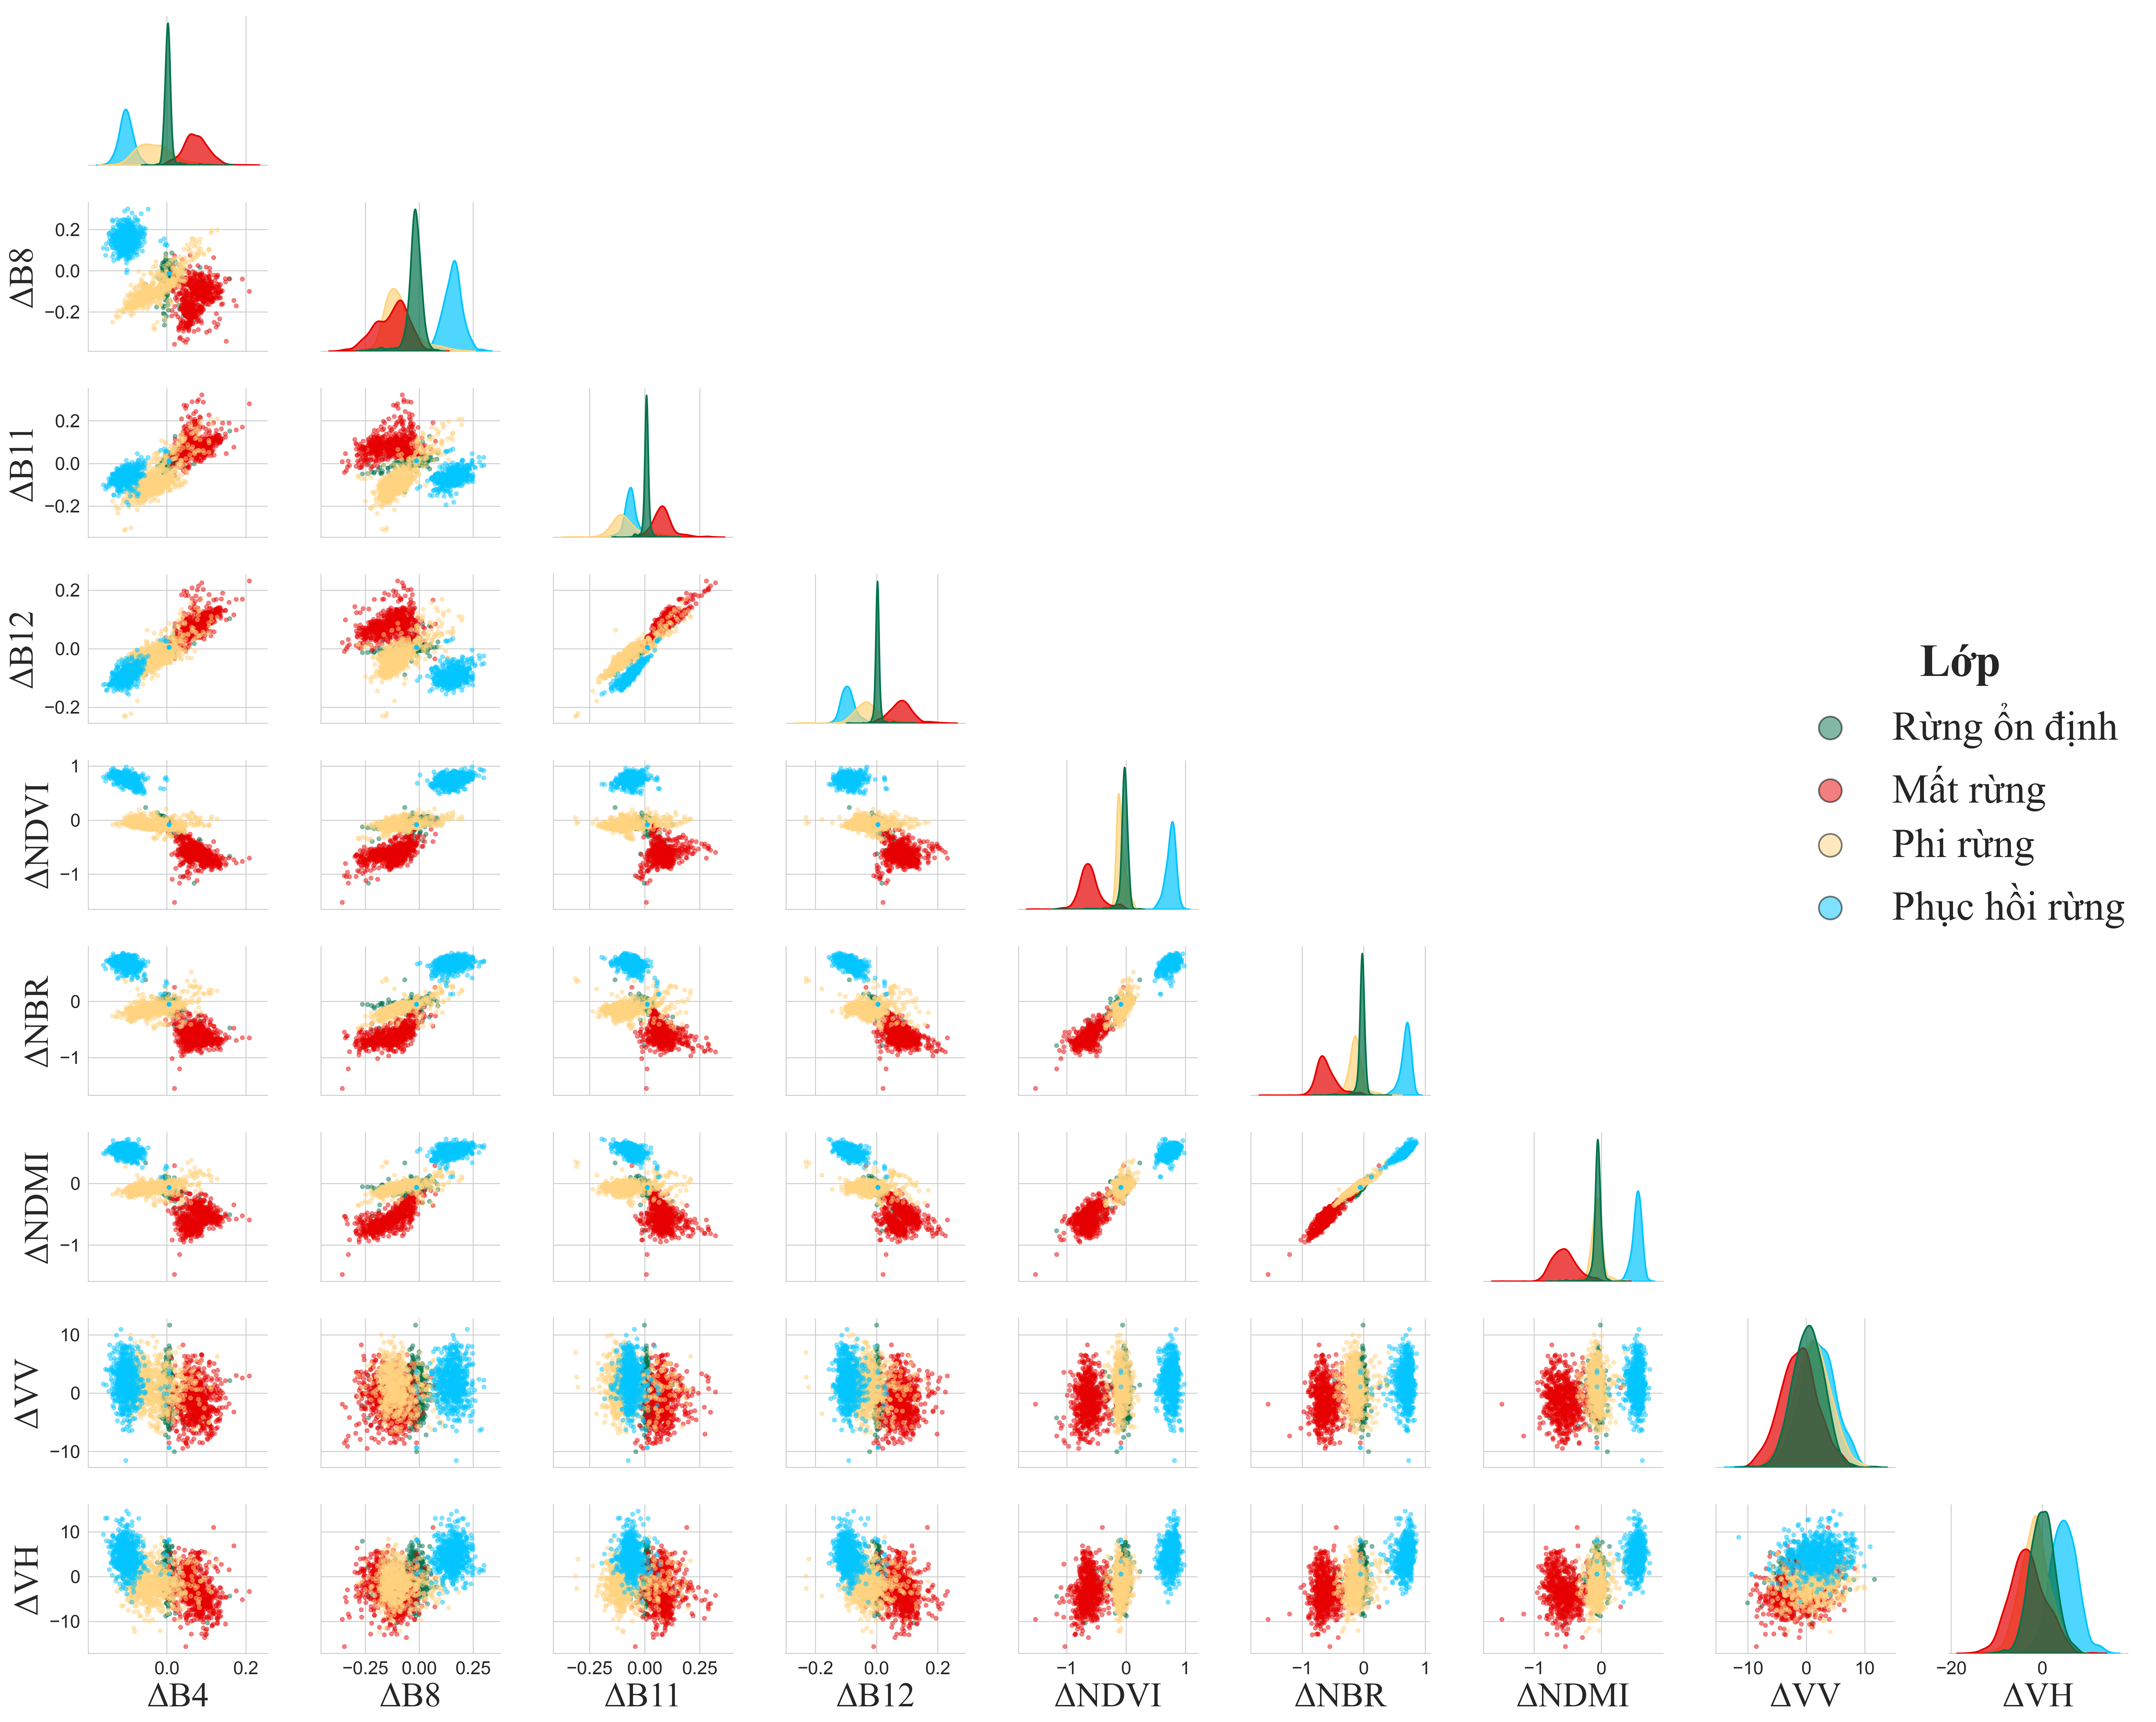
\includegraphics[width=0.95\textwidth]{img/chapter3/pairplot_delta_features.png}
    \caption{Phân bố các đặc trưng delta theo lớp biến động rừng}
    \label{fig:pairplot_delta}
\end{figure}

\subsection{Phương pháp nghiên cứu}

\subsubsection{Chiến lược lấy mẫu và chuẩn bị dữ liệu}
Quy trình chuẩn bị dữ liệu huấn luyện được thực hiện cẩn trọng để đảm bảo tính đại diện và khách quan. Dữ liệu thực địa gồm 2.630 điểm mẫu được thu thập và dán nhãn thủ công cho bốn lớp đối tượng: Rừng ổn định, Mất rừng, Phi rừng và Phục hồi rừng. Các điểm mẫu này được phân bố đều trên toàn vùng nghiên cứu để tránh thiên lệch không gian.

\begin{table}[H]
\centering
\caption{Thống kê dữ liệu thực địa theo lớp biến động}
\label{tab:ground_truth}
\begin{tabular}{|c|l|c|c|l|}
\hline
\textbf{Lớp} & \textbf{Tên} & \textbf{Số điểm} & \textbf{Tỷ lệ} & \textbf{Mô tả} \\
\hline
0 & Rừng ổn định & 656 & 24,9\% & Có rừng ở cả 2 kỳ \\
\hline
1 & Mất rừng & 650 & 24,7\% & Có rừng $\rightarrow$ không có rừng \\
\hline
2 & Phi rừng & 664 & 25,3\% & Không có rừng ở cả 2 kỳ \\
\hline
3 & Phục hồi rừng & 660 & 25,1\% & Không có $\rightarrow$ có rừng \\
\hline
\textbf{Tổng} & & \textbf{2.630} & \textbf{100\%} & Phân bố cân bằng \\
\hline
\end{tabular}
\end{table}

\begin{figure}[H]
\centering
\includegraphics[width=0.9\textwidth]{chapter3/samples.png}
\caption{Bản đồ phân bố không gian các điểm dữ liệu thực địa trên khu vực nghiên cứu tỉnh Cà Mau}
\label{fig:ground_truth_map}
\end{figure}

Để khai thác thông tin ngữ cảnh không gian, thay vì phân loại từng điểm ảnh độc lập, nghiên cứu sử dụng phương pháp trích xuất các ô (patch) kích thước $3 \times 3$ điểm ảnh xung quanh mỗi điểm mẫu. Như vậy, mỗi mẫu dữ liệu đầu vào là một khối tensor có kích thước $(27, 3, 3)$. Trước khi đưa vào mô hình, toàn bộ dữ liệu được chuẩn hóa theo phương pháp Z-score (trừ đi trung bình và chia cho độ lệch chuẩn) để đưa các đặc trưng về cùng một thang đo, giúp quá trình tối ưu hóa hội tụ nhanh hơn.

Dữ liệu được chia thành hai tập độc lập: tập huấn luyện/kiểm định (80\%) và tập kiểm tra (20\%). Việc phân chia được thực hiện theo phương pháp phân tầng (stratified sampling) để đảm bảo tỷ lệ các lớp trong mỗi tập con tương đương với tập dữ liệu gốc. Tập kiểm tra được giữ hoàn toàn riêng biệt và chỉ được sử dụng một lần duy nhất để đánh giá hiệu năng cuối cùng của mô hình.

\subsubsection{Kiến trúc mô hình CNN đề xuất}
Nghiên cứu đề xuất một kiến trúc mạng nơ-ron tích chập (CNN) được thiết kế riêng (custom architecture) cho bài toán này, tối ưu hóa sự cân bằng giữa độ chính xác và chi phí tính toán. Kiến trúc mạng bao gồm các thành phần chính sau:

Khối tích chập đầu tiên bao gồm lớp tích chập (Convolution) với 64 bộ lọc kích thước $3 \times 3$, tiếp theo là lớp chuẩn hóa theo lô (Batch Normalization) và hàm kích hoạt ReLU. Lớp tích chập này có nhiệm vụ trích xuất các đặc trưng không gian và quang phổ sơ cấp từ dữ liệu đầu vào. Ngay sau đó là lớp Dropout 2D với tỷ lệ 0.7, giúp ngắt ngẫu nhiên các kết nối để ngăn ngừa hiện tượng quá khớp (overfitting) - một vấn đề thường gặp khi huấn luyện mạng sâu trên tập dữ liệu nhỏ.

Khối tích chập thứ hai sử dụng 32 bộ lọc để tiếp tục tinh chế các đặc trưng ở mức độ trừu tượng cao hơn, đồng thời giảm chiều dữ liệu để nén thông tin. Cấu trúc của khối này tương tự khối đầu tiên vời đầy đủ các thành phần chuẩn hóa và kích hoạt.

Điểm đặc biệt của kiến trúc này là việc sử dụng lớp Global Average Pooling (GAP) ở giai đoạn cuối thay vì làm phẳng (flatten) toàn bộ tensor. GAP tính trung bình giá trị của mỗi bản đồ đặc trưng, giúp giảm mạnh số lượng tham số của mô hình và tăng khả năng bất biến đối với các dịch chuyển nhỏ trong ảnh. Cuối cùng, các đặc trưng được đưa qua các lớp kết nối đầy đủ (Fully Connected) để thực hiện phân loại vào 4 lớp mục tiêu. Tổng số tham số của mô hình chỉ khoảng 36.676, đảm bảo mô hình gọn nhẹ (lightweight) và có thể huấn luyện nhanh chóng trên phần cứng thông dụng.

\subsection{Kết quả thực nghiệm và thảo luận}

\subsubsection{Đánh giá ảnh hưởng của tham số và nguồn dữ liệu}
Trước khi huấn luyện mô hình cuối cùng, một loạt các thí nghiệm đã được thực hiện để lựa chọn tham số tối ưu. Kết quả so sánh các kích thước patch khác nhau (1x1, 3x3, 5x5, 7x7) cho thấy kích thước 3x3 mang lại hiệu suất cao nhất với độ chính xác 98,86\%. Kích thước này đủ lớn để nắm bắt ngữ cảnh không gian cục bộ nhưng cũng đủ nhỏ để tránh nhiễu từ các đối tượng lân cận không liên quan.

\begin{table}[H]
\centering
\caption{So sánh các kích thước patch}
\label{tab:patch_size}
\begin{tabular}{|c|c|c|c|c|}
\hline
\textbf{Kích thước patch} & \textbf{Accuracy} & \textbf{ROC-AUC} & \textbf{Thời gian huấn luyện} & \textbf{Số tham số} \\
\hline
1×1 & 98,23\% & 99,78\% & 12,5s & 25.348 \\
\hline
\textbf{3×3 (nghiên cứu này)} & \textbf{98,86\%} & \textbf{99,98\%} & 15,2s & 36.676 \\
\hline
5×5 & 98,67\% & 99,89\% & 28,3s & 52.484 \\
\hline
7×7 & 98,29\% & 99,86\% & 41,2s & 71.108 \\
\hline
\end{tabular}
\end{table}

\begin{figure}[H]
    \centering
    \begin{tikzpicture}
        \begin{axis}[
            ybar,
            width=0.85\textwidth,
            height=7cm,
            ylabel={Accuracy (\%)},
            xlabel={Kích thước patch},
            symbolic x coords={1x1, 3x3, 5x5, 7x7},
            xtick=data,
            ymin=97.5,
            ymax=99.5,
            bar width=25pt,
            nodes near coords,
            nodes near coords align={vertical},
            every node near coord/.append style={font=\scriptsize},
            enlarge x limits=0.2,
        ]
        \addplot[fill=blue!60] coordinates {
            (1x1, 98.23)
            (3x3, 98.86)
            (5x5, 98.67)
            (7x7, 98.29)
        };
        \end{axis}
    \end{tikzpicture}
    \caption{So sánh Accuracy theo các kích thước patch}
    \label{fig:patch_size_comparison}
\end{figure}

Nghiên cứu cũng tiến hành đánh giá vai trò của từng nguồn dữ liệu thông qua phương pháp loại trừ (ablation study). Kết quả chỉ ra rằng nếu chỉ sử dụng đơn lẻ dữ liệu quang học Sentinel-2, độ chính xác chỉ đạt 93,42\%. Khi kết hợp thêm dữ liệu radar Sentinel-1, độ chính xác tăng vọt lên 98,86\%. Điều này khẳng định giả thuyết ban đầu rằng sự kết hợp dữ liệu đa nguồn mang lại thông tin bổ sung quan trọng: tín hiệu quang học phản ánh đặc tính sinh học của lá cây, trong khi tín hiệu radar phản ánh cấu trúc vật lý của thân và tán rừng.

\begin{table}[H]
\centering
\caption{Nghiên cứu loại trừ các nguồn dữ liệu}
\label{tab:data_sources}
\begin{tabular}{|l|c|c|c|}
\hline
\textbf{Cấu hình} & \textbf{Số đặc trưng} & \textbf{Accuracy} & \textbf{ROC-AUC} \\
\hline
Chỉ Sentinel-2 (delta) & 7 & 87,65\% & 94,12\% \\
\hline
Sentinel-2 (trước + sau + delta) & 21 & 93,42\% & 97,58\% \\
\hline
Chỉ Sentinel-1 (trước + sau + delta) & 6 & 83,27\% & 91,45\% \\
\hline
\textbf{S1 + S2 (tất cả)} & \textbf{27} & \textbf{98,86\%} & \textbf{99,98\%} \\
\hline
\end{tabular}
\end{table}

\begin{figure}[H]
    \centering
    \begin{tikzpicture}
        \begin{axis}[
            ybar,
            width=0.95\textwidth,
            height=7cm,
            ylabel={Accuracy (\%)},
            symbolic x coords={S2 (delta), S2 (tất cả), S1 (tất cả), S1+S2 (tất cả)},
            xtick=data,
            xticklabel style={rotate=15, anchor=east, font=\small},
            ymin=80,
            ymax=100,
            bar width=22pt,
            nodes near coords,
            nodes near coords align={vertical},
            every node near coord/.append style={font=\scriptsize},
            enlarge x limits=0.15,
        ]
        \addplot[fill=orange!70] coordinates {
            (S2 (delta), 87.65)
            (S2 (tất cả), 93.42)
            (S1 (tất cả), 83.27)
            (S1+S2 (tất cả), 98.86)
        };
        \end{axis}
    \end{tikzpicture}
    \caption{So sánh Accuracy theo các nguồn dữ liệu}
    \label{fig:data_sources_comparison}
\end{figure}

\subsubsection{Hiệu năng mô hình trên tập kiểm tra}
Quá trình huấn luyện sử dụng chiến lược kiểm định chéo 5 phần (5-fold cross-validation) để đảm bảo độ tin cậy. Kết quả trung bình cho thấy độ chính xác ổn định ở mức 98,86\% với độ lệch chuẩn rất thấp, chứng tỏ mô hình không phụ thuộc vào cách chia dữ liệu.

\begin{figure}[H]
\centering
\includegraphics[width=0.95\textwidth]{img/chapter3/cnn_training_history.png}
\caption{Diễn biến loss và accuracy trong quá trình huấn luyện mô hình cuối cùng}
\label{fig:final_training}
\end{figure}

Trên tập kiểm tra độc lập, mô hình đạt độ chính xác toàn cục (Overall Accuracy) là 98,86\% và chỉ số ROC-AUC đạt 99,98\%. Phân tích chi tiết qua ma trận nhầm lẫn (Confusion Matrix) cho thấy mô hình phân loại gần như tuyệt đối chính xác các lớp Phi rừng và Phục hồi rừng (độ chính xác 100\%). Một số ít sự nhầm lẫn (tỷ lệ lỗi khoảng 1.1\%) xảy ra giữa lớp Rừng ổn định và Mất rừng.

\begin{figure}[H]
    \centering
    \begin{tikzpicture}
        % Định nghĩa màu sắc Blues colormap (từ nhạt đến đậm)
        \definecolor{blue0}{RGB}{247,251,255}
        \definecolor{blue1}{RGB}{222,235,247}
        \definecolor{blue2}{RGB}{198,219,239}
        \definecolor{blue3}{RGB}{158,202,225}
        \definecolor{blue4}{RGB}{107,174,214}
        \definecolor{blue5}{RGB}{66,146,198}
        \definecolor{blue6}{RGB}{33,113,181}
        \definecolor{blue7}{RGB}{8,81,156}
        \definecolor{blue8}{RGB}{8,48,107}

        % Kích thước ô
        \def\cellsize{1.8}

        % Các ô với màu Blues gradient
        \fill[blue8] (0*\cellsize, 3*\cellsize) rectangle (1*\cellsize, 4*\cellsize);
        \fill[blue1] (1*\cellsize, 3*\cellsize) rectangle (2*\cellsize, 4*\cellsize);
        \fill[blue0] (2*\cellsize, 3*\cellsize) rectangle (3*\cellsize, 4*\cellsize);
        \fill[blue0] (3*\cellsize, 3*\cellsize) rectangle (4*\cellsize, 4*\cellsize);

        \fill[blue1] (0*\cellsize, 2*\cellsize) rectangle (1*\cellsize, 3*\cellsize);
        \fill[blue8] (1*\cellsize, 2*\cellsize) rectangle (2*\cellsize, 3*\cellsize);
        \fill[blue0] (2*\cellsize, 2*\cellsize) rectangle (3*\cellsize, 3*\cellsize);
        \fill[blue0] (3*\cellsize, 2*\cellsize) rectangle (4*\cellsize, 3*\cellsize);

        \fill[blue0] (0*\cellsize, 1*\cellsize) rectangle (1*\cellsize, 2*\cellsize);
        \fill[blue0] (1*\cellsize, 1*\cellsize) rectangle (2*\cellsize, 2*\cellsize);
        \fill[blue8] (2*\cellsize, 1*\cellsize) rectangle (3*\cellsize, 2*\cellsize);
        \fill[blue0] (3*\cellsize, 1*\cellsize) rectangle (4*\cellsize, 2*\cellsize);

        \fill[blue0] (0*\cellsize, 0*\cellsize) rectangle (1*\cellsize, 1*\cellsize);
        \fill[blue0] (1*\cellsize, 0*\cellsize) rectangle (2*\cellsize, 1*\cellsize);
        \fill[blue0] (2*\cellsize, 0*\cellsize) rectangle (3*\cellsize, 1*\cellsize);
        \fill[blue8] (3*\cellsize, 0*\cellsize) rectangle (4*\cellsize, 1*\cellsize);

        % Vẽ đường viền
        \draw[white, line width=1pt] (0,0) grid[step=\cellsize] (4*\cellsize, 4*\cellsize);

        % Số liệu
        \node[font=\normalsize\bfseries, text=white] at (0.5*\cellsize, 3.5*\cellsize) {129};
        \node[font=\normalsize, text=black] at (1.5*\cellsize, 3.5*\cellsize) {2};
        \node[font=\normalsize, text=black] at (2.5*\cellsize, 3.5*\cellsize) {0};
        \node[font=\normalsize, text=black] at (3.5*\cellsize, 3.5*\cellsize) {0};

        \node[font=\normalsize, text=black] at (0.5*\cellsize, 2.5*\cellsize) {4};
        \node[font=\normalsize\bfseries, text=white] at (1.5*\cellsize, 2.5*\cellsize) {126};
        \node[font=\normalsize, text=black] at (2.5*\cellsize, 2.5*\cellsize) {0};
        \node[font=\normalsize, text=black] at (3.5*\cellsize, 2.5*\cellsize) {0};

        \node[font=\normalsize, text=black] at (0.5*\cellsize, 1.5*\cellsize) {0};
        \node[font=\normalsize, text=black] at (1.5*\cellsize, 1.5*\cellsize) {0};
        \node[font=\normalsize\bfseries, text=white] at (2.5*\cellsize, 1.5*\cellsize) {133};
        \node[font=\normalsize, text=black] at (3.5*\cellsize, 1.5*\cellsize) {0};

        \node[font=\normalsize, text=black] at (0.5*\cellsize, 0.5*\cellsize) {0};
        \node[font=\normalsize, text=black] at (1.5*\cellsize, 0.5*\cellsize) {0};
        \node[font=\normalsize, text=black] at (2.5*\cellsize, 0.5*\cellsize) {0};
        \node[font=\normalsize\bfseries, text=white] at (3.5*\cellsize, 0.5*\cellsize) {132};

        % Nhãn cột (Dự đoán)
        \node[font=\scriptsize, rotate=45, anchor=east] at (0.5*\cellsize, -0.2*\cellsize) {Rừng ổn định};
        \node[font=\scriptsize, rotate=45, anchor=east] at (1.5*\cellsize, -0.2*\cellsize) {Mất rừng};
        \node[font=\scriptsize, rotate=45, anchor=east] at (2.5*\cellsize, -0.2*\cellsize) {Phi rừng};
        \node[font=\scriptsize, rotate=45, anchor=east] at (3.5*\cellsize, -0.2*\cellsize) {Phục hồi rừng};
        \node[font=\small\bfseries] at (2*\cellsize, -1.1*\cellsize) {Dự đoán};

        % Nhãn hàng (Thực tế)
        \node[font=\scriptsize, anchor=east] at (-0.1*\cellsize, 3.5*\cellsize) {Rừng ổn định};
        \node[font=\scriptsize, anchor=east] at (-0.1*\cellsize, 2.5*\cellsize) {Mất rừng};
        \node[font=\scriptsize, anchor=east] at (-0.1*\cellsize, 1.5*\cellsize) {Phi rừng};
        \node[font=\scriptsize, anchor=east] at (-0.1*\cellsize, 0.5*\cellsize) {Phục hồi rừng};
        \node[font=\small\bfseries, rotate=90] at (-1.5*\cellsize, 2*\cellsize) {Thực tế};
    \end{tikzpicture}
    \caption{Ma trận nhầm lẫn trên tập kiểm tra (n=526, Accuracy: 98,86\%)}
    \label{fig:confusion_heatmap}
\end{figure}

Nguyên nhân chủ yếu do các khu vực rừng bị suy thoái nhẹ hoặc mới trồng lại có đặc điểm phổ và cấu trúc chưa rõ ràng, nằm ở ranh giới giữa hai trạng thái này. Tuy nhiên, tỷ lệ lỗi này là hoàn toàn chấp nhận được trong bài toán giám sát diện rộng.

\subsubsection{Kết quả phân loại toàn tỉnh Cà Mau}
Mô hình đã huấn luyện được áp dụng để phân loại toàn bộ khu vực quy hoạch lâm nghiệp tỉnh Cà Mau với diện tích hơn 162.000 ha. Bản đồ kết quả cho thấy diện tích rừng ổn định chiếm phần lớn (khoảng 74,3\%), tập trung chủ yếu ở các khu vực rừng phòng hộ và Vườn Quốc gia Mũi Cà Mau. Diện tích mất rừng được phát hiện khoảng 7.282 ha (tương đương 4,48\%), phân bố rải rác và thường gắn liền với các khu vực ven biển hoặc xen kẽ trong các vùng nuôi trồng thủy sản. Ngược lại, diện tích rừng phục hồi đạt khoảng 4.941 ha (3,04\%).

\begin{figure}[H]
    \centering
    \includegraphics[width=0.95\textwidth]{img/chapter3/Classification.png}
    \caption{Bản đồ phân loại biến động rừng tỉnh Cà Mau}
    \label{fig:classification_map}
\end{figure}

\begin{figure}[H]
    \centering
    \includegraphics[width=0.95\textwidth]{img/chapter3/VQG_Mui_Ca_Mau.png}
    \caption{Bản đồ phân loại biến động rừng khu vực Vườn Quốc gia Mũi Cà Mau}
    \label{fig:vqg_mui_ca_mau}
\end{figure}

Kết quả này cho thấy một xu hướng biến động phức tạp: mặc dù có sự mất mát rừng do các nguyên nhân tự nhiên (sạt lở) và nhân sinh (chuyển đổi mục đích sử dụng), nhưng cũng có những tín hiệu tích cực từ việc phục hồi rừng.

\begin{figure}[H]
    \centering
    \definecolor{stableforest}{HTML}{00734C}
    \definecolor{deforestation}{HTML}{E60000}
    \definecolor{nonforest}{HTML}{FFD37F}
    \definecolor{reforestation}{HTML}{00C5FF}
    \begin{tikzpicture}
        \pie[
            radius=2.5,
            text=legend,
            color={stableforest, deforestation, nonforest, reforestation},
            explode={0, 0.1, 0, 0}
        ]{
            74.30/Rừng ổn định (74{,}30\%),
            4.48/Mất rừng (4{,}48\%),
            18.17/Phi rừng (18{,}17\%),
            3.04/Phục hồi rừng (3{,}04\%)
        }
    \end{tikzpicture}
    \caption{Tỷ lệ diện tích các lớp phân loại}
    \label{fig:pie_chart}
\end{figure}

Bản đồ biến động độ phân giải 10m cung cấp cái nhìn chi tiết chưa từng có, cho phép các nhà quản lý xác định chính xác vị trí các điểm nóng về phá rừng cũng như đánh giá hiệu quả của các dự án trồng rừng. So sánh với các nghiên cứu khác cho thấy phương pháp đề xuất có độ chính xác cạnh tranh cao.

\begin{figure}[H]
    \centering
    \begin{tikzpicture}
        \begin{axis}[
            ybar,
            width=0.9\textwidth,
            height=7cm,
            ylabel={Accuracy (\%)},
            symbolic x coords={Hansen (2013), Ortega (2020), Fayaz (2024), Nghiên cứu này},
            xtick=data,
            xticklabel style={rotate=15, anchor=east, font=\small},
            ymin=80,
            ymax=102,
            bar width=25pt,
            nodes near coords,
            nodes near coords align={vertical},
            every node near coord/.append style={font=\scriptsize},
            enlarge x limits=0.15,
        ]
        \addplot[fill=teal!60] coordinates {
            (Hansen (2013), 85)
            (Ortega (2020), 94)
            (Fayaz (2024), 95.5)
            (Nghiên cứu này, 98.86)
        };
        \end{axis}
    \end{tikzpicture}
    \caption{So sánh Accuracy với các nghiên cứu trước đó}
    \label{fig:literature_comparison}
\end{figure}

